\documentclass[tikz,11pt]{standalone}
\usepackage{lmodern}
\usepackage{amssymb}
\usepackage{pgfplots}
\pgfplotsset{compat=1.17}
\usepgfplotslibrary{external}
\usepgfplotslibrary{groupplots}
\usepgfplotslibrary{fillbetween}
\usetikzlibrary{fadings}
\begin{document}
\tikzsetnextfilename{mvn-dist-lgnd}
\pgfdeclareplotmark{|||}{\pgfpathmoveto{\pgfqpoint{-2pt}{\pgfplotmarksize}}\pgfpathlineto{\pgfqpoint{-2pt}{-\pgfplotmarksize}}\pgfpathmoveto{\pgfqpoint{0pt}{\pgfplotmarksize}}\pgfpathlineto{\pgfqpoint{0pt}{-\pgfplotmarksize}}\pgfpathmoveto{\pgfqpoint{2pt}{\pgfplotmarksize}}\pgfpathlineto{\pgfqpoint{2pt}{-\pgfplotmarksize}}\pgfusepathqstroke}
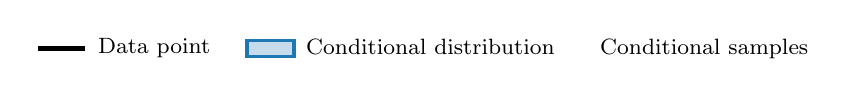
\begin{tikzpicture}
\begin{axis}[hide axis, xmin={0}, xmax={1}, ymin={0}, ymax={1}, legend columns={-1}, legend style={draw={none}, legend cell align={center}, font={\footnotesize}, column sep={0.0625cm}, /tikz/every even column/.append style={column sep=0.375cm}}]
    \addlegendimage{ultra thick}
    \addlegendentry{Data point}
    \addlegendimage{fill opacity={0.25}, area legend, very thick, color={rgb,1:red,0.1216;green,0.4667;blue,0.7059}, fill={rgb,1:red,0.1216;green,0.4667;blue,0.7059}}
    \addlegendentry{Conditional distribution}
    \addlegendimage{only marks, mark={|||}, mark size={3pt}, color={rgb,1:red,0.1216;green,0.4667;blue,0.7059}}
    \addlegendentry{Conditional samples}
\end{axis}
\end{tikzpicture}
\end{document}
